\documentclass[12pt, class=report, crop=false]{standalone}
\usepackage{ba_thesis}

\begin{document}

\chapter{Numerical Methods and Particle in Cell Simulations}%
\label{chap:numerical-methods}

The domain of numerical simulations for laser-plasma interaction is incredibly expansive, with many approaches one can choose from, like numerically solving the Vlasov equation or using Particle-in-cell methods, and many ways to implement and optimize them. I will restrict in this thesis to the second option.

Even so, there are two key integration schemes that sit at the core of a Particle-in-cell software, the Maxwell solver and the particle pusher. In this chapter I aim to analyze in detail the most used schemes and their propeties and eventually give a bird's eye view of the currently available PIC codes out there and the implementation choices they've made.

\section{Numerical Methods}

In this section I aim to summarize the basic theory in the area of numerical methods that would be required to understand the schemes that comprise PIC codes and the problmes they pose. The presentation will be a short review of the concepts developed in the second chapter of the book by~\cite{leimkuhlerSimulatingHamiltonianDynamics2004}.

\subsection{Introduction to Numerical Methods for Solving Differential Equations}

We aim to understand how to find numerical solutions for a system of \(k\) ordinary differential equations with initial condition

\begin{equation}
  \label{eq:ODE}
  \dv{\vb{u}}{t} = \vb{f}(\vb{u}),\; \vb{u}(t_0) = \vb{u_0} \in \mathbb{R}^k\,,
\end{equation}
where \(t_0\) is the initial time, \(\vb{u_0}\) is the initial value of our solution and \(\vb{f}\) is a function that relates the elements in the solution vector. We can always set the time such that we have \(t_0=0\) for simplicity.

We usually refer to the solution \(\vb{u}\) as a trajectory. If the solution can be determined by integration in time starting from an appropriate initiall condition, the differential equation defines a one-parameter group of propagation maps \(\phi_t:\mathbb{R}^k \rightarrow \mathbb{R}^k\). The group properties are given by the property that solving the probem from \(t_0\) to \(t_1\) and then from \(t_1\) to \(t_2\) is the same as solving from \(t_0\) directly to \(t_2\). Thus, the composition of those maps inherits the properties of the addition of real numbers. Note that this is just the \textit{phase flow} of the equation in the way we defined it in~\cref{sec:Vlasov}.

Solving~\cref{eq:ODE} numerically means to discretize the time domain and find a scheme that would be able to propagate within sizable error the trajectory. Thus one obtains a set of values for the solution function at fixed points in time and those values can be eventually interpolated to estimate the values in between them. The simplest way to discretize the domain is to have a fixed small time \(\Delta t\) step such that \(t_1=t_0 + \Delta t\), \(t_2=t_1 + \Delta t\), and so on. More complex discretizations can be done if we know specific properties of the solution or if we are interested to increase the accuracy over some interval at the cost of decreasing it for another interval, but in what follows we will only deal with the simple equidistant discretization.

\subsection{One-Step Methods}
\label{ssec:one-step-m}

In general, one can choose to include at each iteration as many of the previously computed points on the trajectory. For example, if we want to use \(k\) previous points we have to find an appropriate scheme that computes \(\vb{u_{n+1}}\)  in terms of \(\vb{u_{n-k+1}}\), \(\vb{u_{n-k+2}}\),\dots, \(\vb{u_{n}}\) and the corresponding values of the derivative function \(\vb{f}(\vb{u_{n-k+1}})\), \(\vb{f}(\vb{u_{n-k+2}})\),\dots, \(\vb{f}(\vb{u_{n}})\). Here we denoted the point \(\vb{u}(t_i)\) simply by \(\vb{u_i}\). A linear multistep method of order k is, as the name suggests, a linear such reccurence relation. We are interested specifically in linear maps since they can be represented as matrices and under a matrix formalism they are trivial to implement in code.

This subsection is dedicated to one-step methods, that is for the case \(k=1\). We have as such to find an infinitesimal flow map that gives \(\vb{u_{i+1}} = \phi_{\Delta t} \vb{u_{i}}\) for each \(i\). Finding any point on the trajectory is then simply a matter of appling the infinitesimal map multiple times to the initial condition

\begin{equation*}
  \vb{u_{n}} = \phi_{\Delta t}^n \vb{u_{0}}\,.
\end{equation*}
Here I denoted with \(\phi_{\Delta t}^n\) the composition of \(\phi_{\Delta t}\) with itself \(n\) times.

We have the following analitical equation between two consecutive points

\begin{equation}
  \vb{u_{i+1}} - \vb{u_i} = \int_0^{\Delta t} \dd{\tau} \vb{f} (\vb{u}(t_i +\tau))\,.
\end{equation}
In order to find a one step-method we have to approximate the integral with a sum, which is done by using an appropriate quadrature rule

\begin{equation}
  \vb{u_{i+1}} \approx \vb{u_i} + \sum_{j=1}^s b_j \vb{f} (\vb{u}(t_i + \tau_j)) \Delta t\,,
\end{equation}
where \(b_j\) are the weights and \(\tau_j\) are the quadrature points.

Here are some basic examples:

\subsubsection{Explicit Euler Scheme}

Obtained by setting \(s=1\), \(b_1=1\), and \(\tau_1 = 0\).

\begin{equation}
  \vb{u_{i+1}} \approx \vb{u_i} + \vb{f}(\vb{u_i}) \Delta t + \mathcal{O}(\Delta t^2)\,.
\end{equation}

\subsubsection{Implicit Euler Scheme}

Obtained by setting \(s=1\), \(b_1=1\), and \(\tau_1 = \Delta t\).

\begin{equation}
  \vb{u_{i+1}} \approx \vb{u_i} + \vb{f}(\vb{u_{i+1}}) \Delta t + \mathcal{O}(\Delta t^2)\,.
\end{equation}

\subsubsection{Trapezoid Rule}

Obtained by setting \(s=2\), \(b_1=b_2=\frac{1}{2}\), and \(\tau_1 = 0\), \(\tau_2 = \Delta t\).

\begin{equation}
  \vb{u_{i+1}} \approx \vb{u_i} + \frac{1}{2} \left[\vb{f}(\vb{u_{i}}) + \vb{f}(\vb{u_{i+1}}) \right] \Delta t + \mathcal{O}(\Delta t^3)\,.
\end{equation}

\subsubsection{Implicit Midpoint Rule}

Obtained by setting \(s=1\), \(b_1=1\), and \(\tau_1 = \frac{\Delta t}{2}\), using \(\vb{u}\left(t_i+\frac{\Delta t}{2}\right) \approx \frac{1}{2} (\vb{u_i} + \vb{u_{i+1}})\). Numerous more complex methods can be obtained by improving the latter approximation.

\begin{equation}
  \vb{u_{i+1}} \approx \vb{u_i} + \vb{f}\left(\frac{\vb{u_i} + \vb{u_{i+1}}}{2}\right) \Delta t + \mathcal{O}(\Delta t^3)\,.
\end{equation}
\(\blacksquare\)

It is important to note that while there methods are for first order ODE sistems, they can be often employed in higher order ODE systems. For example let us analyze the systems that can arise from Newton's second law

\begin{equation}
  \dv[2]{\vb{r}}{t} = \vb{F}(\vb{r})\,.
\end{equation}
By defining \(\vb{v} = \dv{\vb{r}}{t}\) we can transform it in a system of first order equations

\begin{subequations}
  \begin{align}
    \dv{\vb{v}}{t} = \vb{F}(\vb{r})\\
    \vb{v} = \dv{\vb{r}}{t}\,.
  \end{align}
\end{subequations}
This can be rewritten to look more like~\cref{eq:ODE} through an inspired notation

\begin{subequations}
  \begin{align}
    \vb{u} =
    \begin{bmatrix}
      \vb{r}\\
      \vb{v}
    \end{bmatrix} \\
    \vb{f}(\vb{u}) =
    \begin{bmatrix}
      \vb{v}\\
      \vb{F}(\vb{r})
    \end{bmatrix}\,.
  \end{align}
\end{subequations}

\subsection{Error Estimation}

One of the two main aspects that one needs to study when they propose to use a numerical scheme is accuracy. It basically refers to the error of the numerical solution compared to the real solution.

Error can arise when using the methods described so far from two mechanism: the difference between the approximation used and the Taylor expansion of the function (truncation error), and the accumulation of error caused by the discretization of the trajectory (round off error). The order of a method is defined by the power in the first Taylor coefficient neglected by the scheme minus one. In the examples above, the Euler methods are of order 1, while the Trapezoid and Midpoint Rules have order 2. The oreder of the method shows the dependence of the global error with respect to the step-size of the discretization of the domain. So for an order 1 method, the error is linear in step-size, for an order 2, the error is polynomial in step-size, and so on.

Having all this in mind, making a more accurate numerical scheme is to have the numerical solution just as close to the real solution for a larger time-step, or, conversely, having the numerical solution closer to the real solution for the same step-size.

\subsection{Runge-Kutta Methods}

The Runge-Kutta method is a generalization of the type of methods used before. As such, the schemes given as examples of one-step methods are actually particular cases of the more general Runge-Kutta method. The explicit Runge-Kutta for~\cref{eq:ODE} in particular is the following

\begin{subequations}
  \begin{align}
    \vb{u_{n+1}} = \vb{u_n} + \Delta t \sum_{i=1}^s b_i \vb{f}(\vb{U_i}) \\
    \label{eq:rk}
    \vb{U_i} = \vb{u_n} + \Delta t \sum_{j=1}^s a_{ij} \vb{f}(\vb{U_j}),\; i = \overline{1,s}\\
    a_{i,j}=0\; for\; j\geq i\,.
  \end{align}
\end{subequations}
This time around, each scheme is defined by a choice of \(s\), \(b_i\) weights and the Runge-Kutta matrix \(a_{ij}\). Note that in all our considerations so far related to~\cref{eq:ODE} the function \(\vb{f}\) does not depend on time. This is because we are not interested in that posibility for the purpose of our PIC study. The Boris push propagates the particles over a small time interval while keeping the fields constant, then the Maxwell solver advances the fields in time taking into account the new particle positions. Nonetheless, for the sake of completion, I mention that including the time dependence would mean converting \(\vb{f}(\vb{U_j})\) in~\cref{eq:rk} with \(\vb{f}(t_n + c_i \Delta t, \vb{U_j})\) and \(c_1 =0\). Thus, in order to have a scheme, now we would also need the set of \(c_i\) parameters which are commonly referred to as nodes. The list of all appropriate components for one scheme is presented in literature in Butcher tables. Since each scheme has its own unique table, the numerical properties (accuracy and stability can be computed using the tables. A more in depth explanation on how these tables work can be found in the book by~\cite{butcherNumericalMethodsOrdinary2008}.

\subsection{Leapfrog Algorithm}

In specific situations we can apply the approximation methods disscused so far to separate parts of the solution. This is the mindset for creating partitioned Runge-Kutta methods. As an example, suppose our initial system of ODE (\cref{eq:ODE}) can be separated as such

\begin{subequations}
  \begin{align}
    \dv{\vb{u}}{t} = \vb{f_1}(\vb{u}, \vb{v})\\
    \dv{\vb{v}}{t} = \vb{f_2}(\vb{u}, \vb{v})\,.
  \end{align}
\end{subequations}
To have a partitioned Runge-Kutta scheme we have to use two different regular Runge-Kutta schemes, one for each subset of equations, so to say

\begin{subequations}
  \label{eq:RKN}
  \begin{align}
    \vb{u_{n+1}} = \vb{u_n} + \Delta t \sum_{i=1}^s b_i^u \vb{f_1}(\vb{U_i}, \vb{V_i}) \\
    \vb{v_{n+1}} = \vb{v_n} + \Delta t \sum_{i=1}^s b_i^v \vb{f_2}(\vb{U_i}, \vb{V_i}) \\
    \vb{U_i} = \vb{u_n} + \Delta t \sum_{j=1}^s a_{ij}^u \vb{f_1}(\vb{U_i}, \vb{V_i}),\; i = \overline{1,s}\\
    \vb{V_i} = \vb{v_n} + \Delta t \sum_{j=1}^s a_{ij}^v \vb{f_2}(\vb{U_i}, \vb{V_i}),\; i = \overline{1,s}\,.
  \end{align}
\end{subequations}

In the perspective of the discussion at the end of \cref{ssec:one-step-m}, we can see that this method is useful in solving equations of motion described by Newton's second law. In this context, the scheme in~(\ref{eq:RKN}) is refered to as a Runge-Kutta-Nyström method.

In our endeavours, for equations of the form

\begin{subequations}
  \begin{align}
    \dv{\vb{r}}{t} = \vb{v}\\
    M\dv{\vb{v}}{t} = - \grad_{\vb{r}} V(\vb{r})\,,
  \end{align}
\end{subequations}
we are interested in the Störmer-Verlet method

\begin{subequations}
  \begin{align}
    \label{eq:SV-1}
    \vb{r_{n+1}} = \vb{r_n} +\Delta t \vb{v_{n+\frac{1}{2}}}\\
    \label{eq:SV-2}
    M\vb{v_{n+\frac{1}{2}}} = M\vb{v_n} - \frac{\Delta t}{2} \grad_{\vb{r}} V(\vb{r_n})\\
    \label{eq:SV-3}
    M\vb{v_{n+1}} = M\vb{v_{n+\frac{1}{2}}} - \frac{\Delta t}{2} \grad_{\vb{r}} V(\vb{r_{n+1}})\,.
  \end{align}
\end{subequations}

A different scheme can be derived by playing around with the realations of this method. From~\cref{eq:SV-1} we can extract the mid-step velocity as

\begin{subequations}
  \label{eq:mid-step-v}
  \begin{align}
    \vb{v_{n+\frac{1}{2}}} = \frac{\vb{r_{n+1}} - \vb{r_n}}{\Delta t}\\
    \vb{v_{n-\frac{1}{2}}} = \frac{\vb{r_n} - \vb{r_{n-1}}}{\Delta t}\,,
  \end{align}
\end{subequations}
for two consecutive steps. By lowering~\cref{eq:SV-3} with 1, we have

\begin{equation}
  M\vb{v_{n}} = M\vb{v_{n-\frac{1}{2}}} - \frac{\Delta t}{2} \grad_{\vb{r}} V(\vb{r_{n}})\,,
\end{equation}
which replaced in~\cref{eq:SV-2} gives a reccurence relation for the mid-step velocity

\begin{equation}
  M\frac{\vb{v_{n+\frac{1}{2}}} - \vb{v_{n-\frac{1}{2}}}}{\Delta t} = - \grad_{\vb{r}} V(\vb{r_n})\,.
\end{equation}
We now insert in this~\cref{eq:mid-step-v} to finally obtain the leapfrog scheme

\begin{equation}
  M\frac{\vb{r_{n+1}} - 2\vb{r_n} + \vb{r_{n-1}}}{\Delta t^2} = - \grad_{\vb{r}} V(\vb{r_n})\,.
\end{equation}

Since these two schemes are closely connected by~\cref{eq:mid-step-v}, they have the same order. Since I haven't really given an example so far for how one can find the order of a numerical scheme, I will present in the following the proof for the fact that the leapfrog method is of second ordrer.

Let us expand the position function in two ways around a fixed moment in time \(t\)

\begin{subequations}
  \begin{align}
    \vb{r}(t+\Delta t) = \vb{r}(t)+ \dv{\vb{r}(t)}{t} \frac{\Delta t}{1!}+ \dv[2]{\vb{r}(t)}{t} \frac{\Delta t^2}{2!} + \dv[3]{\vb{r}(t)}{t} \frac{\Delta t^3}{3!}+ \mathcal{O}(\Delta t^4)\\
    \vb{r}(t-\Delta t) = \vb{r}(t)- \dv{\vb{r}(t)}{t} \frac{\Delta t}{1!}+ \dv[2]{\vb{r}(t)}{t} \frac{\Delta t^2}{2!} - \dv[3]{\vb{r}(t)}{t} \frac{\Delta t^3}{3!}+ \mathcal{O}(\Delta t^4)\,.
  \end{align}
\end{subequations}
Adding these up we have

\begin{equation}
  \vb{r}(t+\Delta t) + \vb{r}(t-\Delta t)= \vb{r}(t)+ \dv[2]{\vb{r}(t)}{t} \Delta t^2 + \mathcal{O}(\Delta t^4)\,,
\end{equation}
or, moving the derivative to the left and dividing by \(\Delta t^2\)

\begin{equation}
  \dv[2]{\vb{r}(t)}{t} = \frac{\vb{r}(t+\Delta t) - 2 \vb{r}(t) + \vb{r}(t-\Delta t)}{\Delta t^2} + \mathcal{O}(\Delta t^2)\,.
\end{equation}
Note that we just recovered the second derivative approximation that generates the leapfrog scheme, so our proof is finished.

\subsection{Stability}

In order to understand the concept of stability, let us study the behaviour of some integration schemes in solving the most basic and the most important system of equations in physics -- the linear harmonic oscillator

\begin{subequations}
  \label{eq:HO}
  \begin{align}
    \dv{x}{t} = v\\
    \dv{v}{t} = -\omega^2 x\,.
  \end{align}
\end{subequations}

The figure below ilustrates the phase space representation of the solutions obtained via five different numerical methods (with the frequency set to 1 for simplicity). The plots of the analytic solution is given as well for reference. The Julia code used for these small simulations can be found in the Appendix for the reader interested in seeing and example on how to use these methods in parctice.

\begin{figure}[h]
  \centering
  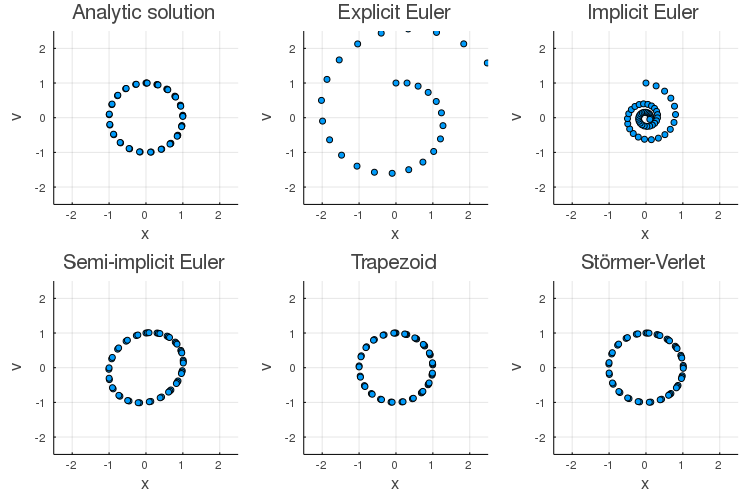
\includegraphics[width=0.85\textwidth]{stability_plots}%
  \caption{Phase space plots of the solution for the harmonic oscillator equations using different numerical methods. The angular frequency is \(\omega =1\), the total time of the simulation is 15 and the time-step is 0.3.}\label{fig:stability}%
\end{figure}

We can see a clear distinction in the solutions obtained. The trapezoid method and Störmer-Verlet method are very close to the real circular solution. On the oposite spectrum, the mplicit and explicit Euler methods show a clearly undesired behaviour, much different from the others. The semi-implicit Euler methods does a decent job, but the shape is a bit oblate. Even so, this scheme has a useful property, namely it is volume preserving. This means that the volume in phase space of the solution obtained is constant over an arbitrarily large number of periods. In contrast, the phase space volume of the implicit and explicit Euler integrators isn't even well defined because the solution diverges too fast. The difference though does not lay in volume preservence, but in what we call \textit{asimptotic stability}. The best way to study this property is mathematically. While a picture like that in~\cref{fig:stability} gives a good visual hint to what asimptotic stability of a scheme is, it was especially exagerated by choosing a large time-step. If one reruns those simulations with a time step of 0.01 instead of 0.3, almost all plots will start looking like a circle. That doesn't mean that we fixed our methods, but rather that by increasing the accuracy we made the imperfections manifest over a much larger time scale. Indeed, if we increase the total duration of the simulation enough, we would see that thing are still bad for the first two Euler methods. This is shown in~\cref{fig:stability2}.

\begin{figure}[h]
  \centering
  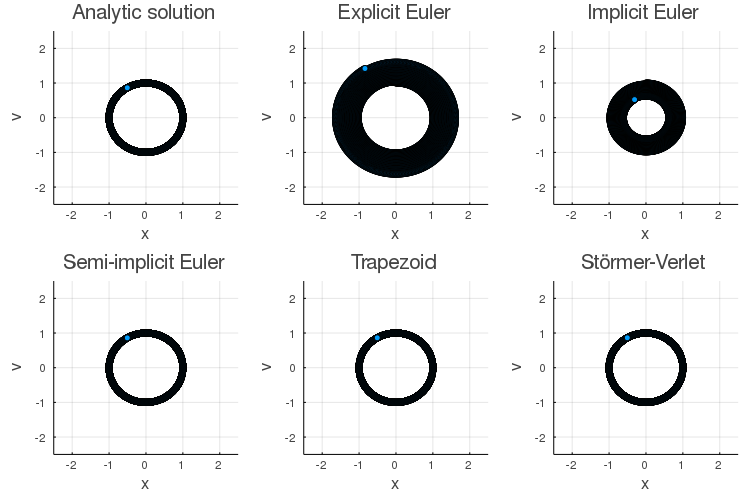
\includegraphics[width=0.85\textwidth]{stability_plots2}%
  \caption{Phase space plots of the solution for the harmonic oscillator equations using different numerical methods. The angular frequency is \(\omega =1\),  but this time around the total time of the simulation is 100 and the time-step is 0.01.}\label{fig:stability2}%
\end{figure}

So how can we study this asimptotic stability? Let us rewrite the linear harmonic oscillator~\cref{eq:HO} in matrix form

\begin{equation}
  \dv{t}
  \begin{bmatrix}
    x\\ v
  \end{bmatrix}
  =
  \begin{bmatrix}
    0 & 1\\
    -\omega^2 & 0
  \end{bmatrix}
  \begin{bmatrix}
    x\\ v
  \end{bmatrix}\,.
\end{equation}
We can actually do better that this and find a flow chart, since we know the most general analytic solution for our problem

\begin{subequations}
  \begin{align}
    x = A \sin(\omega t) + B \cos(\omega t)\\
    v = \omega A \cos(\omega t) -  \omega B \sin(\omega t)\,.
  \end{align}
\end{subequations}
At time \(t=0\) these equations become simply \(x_0 = B\) and \(v_0 = \omega A\). So, using the initial conditions we now have

\begin{subequations}
  \begin{align}
    x = x_0 \cos(\omega t) + v_0 \frac{1}{\omega} \sin(\omega t)\\
    v = - x_0 \omega \sin(\omega t) + v_0 \cos(\omega t)\,,
  \end{align}
\end{subequations}
or, in matrix form

\begin{subequations}
  \begin{align}
  \begin{bmatrix}
    x\\ v
  \end{bmatrix}
  =
  \begin{bmatrix}
    \cos(\omega t) & \frac{1}{\omega} \sin(\omega t)\\
    -\omega \sin(\omega t)  & \cos(\omega t)
  \end{bmatrix}
  \begin{bmatrix}
    x_0\\ v_0
  \end{bmatrix} \\
  \phi_t = \begin{bmatrix}
    \cos(\omega t) & \frac{1}{\omega} \sin(\omega t)\\
    -\omega \sin(\omega t)  & \cos(\omega t)
  \end{bmatrix}\,,
  \end{align}
\end{subequations}
where we denoted by \(\phi_t\) the analytical flow map. There is a new way to see numerical methods now. Coming up with a new scheme is equivalent to finding a different approximation for the infinitesimal version of this map. But befor we delve into this topic, let us fing the eigenvalues of \(\phi_t\). The computation is quite straightforward

\begin{equation*}
  \lambda \begin{bmatrix}
    x_0\\ v_0
  \end{bmatrix}
  =
  \begin{bmatrix}
    \cos(\omega t) & \frac{1}{\omega} \sin(\omega t)\\
    -\omega \sin(\omega t)  & \cos(\omega t)
  \end{bmatrix}
  \begin{bmatrix}
    x_0\\ v_0
  \end{bmatrix}
\end{equation*}

\begin{equation*}
  v_0(\lambda - \cos(\omega t)) = - x_0 \omega \sin(\omega t)
\end{equation*}
\begin{equation*}
  v_0\frac{1}{\omega} \sin(\omega t) = x_0 (\lambda - \cos(\omega t)) \,.
\end{equation*}
Dividing these last two equations gives

\begin{equation*}
  (\lambda - \cos(\omega t))^2 = - \sin[2](\omega t)
\end{equation*}
\begin{equation*}
  \Rightarrow \lambda^2 - 2\lambda \cos(\omega t) +1 = 0\,,
\end{equation*}
which gives the solution

\begin{equation}
  \lambda_{1,2} = \ee^{\pm \ii \omega t}\,.
\end{equation}
Now let us look at the methods. The explicit Euler method has the following infinitesimal flow map and its eigenvalues

\begin{subequations}
  \begin{align}
  \phi_{\Delta t}^{Euler} =
  \begin{bmatrix}
    1 & \Delta t \\
    -\omega^2 \Delta t & 1
  \end{bmatrix}\\
  \lambda_{1,2}^{Euler} = 1 \pm \ii \omega \Delta t\,,
  \end{align}
\end{subequations}
which is obviously just a fisrt order approximation of \(\phi_t\) and its eigenvalues. Now we can give the definition of stability and see why this scheme is not stable for our problem.

\begin{definition}
  A numerical method is stable if the solution it gives for a linear problem has an asimptotically bounded growth.
\end{definition}

This basically assures that the error does not blow up. While this is an intuitive definition, there is a beter way to go about things mathematically. Without going into details about forward and backward stability, we can mention the concept of mixed stability. The idea is the following: looking at~\cref{eq:ODE} let us take \(\vb{f}\) be the analytic propagation function and \(\vb{\tilde{f}}\) the one given by the scheme, while \(\vb{z}\) and \(\vb{\tilde{z}}\) are the analytic and numeric solution, respectively, at the same point in time. The method has mixed stability if the quantity \(\frac{\norm{\vb{\tilde{f}}(\vb{z}) - \vb{f}(\vb{\tilde{z}})}}{\vb{f}(\vb{\tilde{z}})}\) is within machine error for an \(\vb{\tilde{z}}\) with relative error within machine error.

For the interested reader, a list of relevant mathematical definitions related to stability can be found in the presentation by~\cite{liuConditioningNumericalStability}. However, we will restric ourselves to an important and powerful result. The growth of the error after applying the infinitesimal flow map \(n\) is proportional to the \(n^{th}\) power of the corresponding eigenvalues. In this context we can formulate the following theorem.

\begin{theorem}
  A suficient condition for a method to have asimptotic stability is to have the eigenvalues of it's matrix laying in the closed unit disc (unit circle included) in the complex plane, and, if any eigenvalue lies on the unit circle it must be simple (not repeated).
\end{theorem}

A quick look at \(\lambda_{1,2}^{Euler}\) reveals that their modulus is larger than 1. Because of this, the growth of the error in the explicit Euler method is exponential. In fact, in this case, there is no time-step we can choose to make it stable. A point has to be made though: imstability does not deny convergence. As discussed in the beginning of the section, depending on how small of a time-step we choose for a specific simulation duration we can make the instability effects negligible. But this can come at a cost of computational power. Stable algoithms are useful in the way that we can reduce the strain on our computer without obtaining diverging errors.

As we saw in the begining of this section, there are other methods that are stable for the linear harmonic oscillator problem. However, an unconditionally stable scheme is hard to come about. Most of the time we can find a certain condition for our method to be stable. As an example, let us look at the Störmer-Verlet method.

In the context of~\cref{eq:HO}, \cref{eq:SV-1,eq:SV-2,eq:SV-3} become

\begin{subequations}
  \begin{align}
    x_{n+1} = x_n + v_{n+\frac{1}{2}} \Delta t\\
    v_{n+\frac{1}{2}} = v_{n} - x_n \frac{\omega^2 \Delta t}{2} \\
    v_{n+1} = v_{n+\frac{1}{2}} - x_{n+1} \frac{\omega^2 \Delta t}{2}\,,
  \end{align}
\end{subequations}
or

\begin{subequations}
  \begin{align}
    x_{n+1} = x_n \left( 1 - \frac{\omega^2 \Delta t^2}{2} \right) + v_n \Delta t\\
    v_{n+1} = - x_n \left(1 - \frac{\omega^2 \Delta t^2}{4}\right) \omega^2 \Delta t + v_n \left( 1 - \frac{\omega^2 \Delta t^2}{2} \right)\,,
  \end{align}
\end{subequations}
which gives the infinitesimal flow map

\begin{equation}
  \phi_{\Delta t}^{SV} =
  \begin{bmatrix}
    1 - \frac{\omega^2 \Delta t^2}{2} & \Delta t\\
    - \left(1 - \frac{\omega^2 \Delta t^2}{4}\right) \omega^2 \Delta t & 1 - \frac{\omega^2 \Delta t^2}{2}
  \end{bmatrix}\,.
\end{equation}
In order to make solving for eigenvalues easier let us employ the notation \(\eta = \frac{\omega^2 \Delta t^2}{2}\). Then, we have

\begin{subequations}
  \begin{align}
    \lambda x_0 = x_0 (1-\eta) + v_0 \Delta t\\
    \lambda v_0 = - 2 \frac{x_0}{\Delta t} \eta \left(1-\frac{\eta}{2}\right) + v_0 (1-\eta)\,,
  \end{align}
\end{subequations}
followed by

\begin{subequations}
  \begin{align}
    x_0 (\lambda + \eta -1) = v_0 \Delta t\\
    2 x_0 \eta \left(1-\frac{\eta}{2}\right) = - (\lambda + \eta -1)v_0 \Delta t\,.
  \end{align}
\end{subequations}
Dividing these leads to the final equation for the eigenvalues

\begin{equation}
  \lambda^2 - 2(1-\eta) \lambda +1 = 0\,.
\end{equation}
The discriminant of this equation is \(4\eta(\eta-2)\) and, consequently, the eigenvalues are

\begin{equation}
  \lambda_{1,2} = 1 - \eta \pm \sqrt{\eta(\eta - 2)}\,.
\end{equation}
Note that their product is 1. We are now interested in the modulus of these. For \(\eta> 2\) the solutions are real and the modulus of one of them is easily found to be greater than unity. Indeed, if \(\eta = 2+\alpha\), \(\alpha>1\)

\begin{equation}
  \abs{\lambda_{1,2}} = \abs{1-\eta \pm \sqrt{\eta(\eta-2)}} = \abs{-1 - (\alpha \mp \sqrt{\alpha^2 + 2\alpha})} >1\,,
\end{equation}
since \(\alpha + \sqrt{\alpha^2 + 2\alpha} > 0\). If \(\eta< 2\) the eigenvalues are complex and are conjucates of each other, such that their modulus is 1. Thus, we conclude that the method is stable for \(\eta< 2\), which translates to

\begin{equation}
  \Delta t < \frac{2}{\omega} = \frac{T}{\pi}\,.
\end{equation}

\section{The Relevant Equations}

Particle-in-cell codes are nowadays the most popular popular tool for simulating plasma systems. One of the best references for what they are, how they work and how reliable the results are is the book by~\cite{birdsallPlasmaPhysicsComputer1995}, which describes the main numerical methods used and some of their properties. However, Particle-in-cell codes have evolved greatly in the last two decades and new techniques and optimizations have been produced and even put in practice. Even so, with the exception of quasistatic codes, they are still involved in solving the same physical equations. As such, it is useful for anyone interested in working with such software to know and understand the principles behind.

In general, PIC codes have four main componets:
\begin{enumerate}
  \item A Maxwell solver which propagates the Maxwell equations (which are relativistic invariant by themselves) in time and space on the grid
  \begin{subequations}
    \begin{align}
    \div{\vb{E}} & = \frac{\rho}{\varepsilon_0} \\
    \div{\vb{B}} & = 0 \\
    \curl{\vb{E}} & = - \pdv{\vb{B}}{t} \\
    \curl{\vb{B}} & = \mu_0 \vb{j} + \frac{1}{c^2} \pdv{\vb{E}}{t} \,;
    \end{align}
  \end{subequations}
  \item A field gatherer that interpolates the electromagnetic field at the particle positions on the grid;
  \item A particle pusher that advances the positions and velocities of each particle under the action of the Lorentz force (which we will write in its relativistic form)
  \begin{subequations}
    \begin{align}
      \label{eq:NL}
      \dv{\vb{p_\alpha}}{t} = q_\alpha \left(\vb{E}+\frac{\vb{p_\alpha}}{m_\alpha \gamma_\alpha} \cp \vb{B} \right)\\
      \gamma_\alpha = \sqrt{1+\left(\frac{\vb{p_\alpha}}{m_\alpha c}\right)^2}\,,
    \end{align}
  \end{subequations}
  where \(\alpha\) indexes each particle;
  \item Acurrent and charge depositor which computes the current and charge densities on the grid by interpolating the particle distributions.
\end{enumerate}

The main appeal of this approach is its self-consistency. That is, the total fields used are both those that are part of the electromagnetic waves that are introduced in the system (in general laser beams) and those generated by the charged particles that compose the plasma. As such we also include the long range Coulombian interaction between particles. The short range interaction, namely collisions between particles, is by default neglected since we usually simulate rarefied plasmas, but many codes now come with additional routines that include these processes. Additional routines are now developed with the advent of the high intensity laser technologies because at the corresponding energies reached by the particles quantum electrodynamical effects become relevant. Although there are quite a few PIC codes that include QED routines, there is still a long way untill these algorithms reach the efficiency and stability that of those four main ones described above. As such, the implementation of QED effects in numerical plasma simulations is currently a hot research topic.

It is mandatory to mention that while the four steps above outline a microscopic model, PIC simulations are not completely microscopic due to technological limitations regarding computing power. Instead of working with one virtual particle for one real particle, it is customary to use macro-particles. A macro-particle represents many particles of the same species (from \(10^6\) to \(10^11\) depending on the propeties of our plasma) moving colectively. These particles are obviously not localized at a single point, but rather they have a shape function attached to them to make the derivation of currents and charge densities more consistent. For a long time the use of macro-particles was not supported by argument and was a source of criticism towards PIC methods. The defense was built only on the excuse of that the simulations give very accurate statistical results. Things are different nowadays. We can now explain (quite easily in fact) that the macro-particles themselves can be interpreted a statistical ensamble of real particles. The secret lies in the Vlasov equation.

\subsection{The Connection with the Vlasov Equation}

Let us revisit the Vlasov equation, which we derived in~\cref{sec:Vlasov}

\begin{equation}
  \pdv{\rho}{t} + \vb{f}\vdot\pdv{\rho}{\vb{p}} + \vb{v}\vdot\pdv{\rho}{\vb{r}} = 0\,,
\end{equation}
where \(\rho\) was the distribution function that describes the entire system of particles, \(\vb{p}=(\vb{p_1}, \vb{p_2},\dots )\) and \(\vb{v}=(\vb{v_1}, \vb{v_2},\dots )\), \(\vb{r}=(\vb{r_1}, \vb{r_2},\dots )\) the momenta, the velocities, and the positions of the particles, and \(\vb{f}=(\vb{f_1}, \vb{f_2},\dots )\) the forces acting on each particle.

The main argument in the following discussion is a relativistic upgrade of the one in~\cite{liuHighPowerLaserPlasmaInteraction2020}. For consistency with the equations we outlined for the PIC method, I rewrite this equation in its relativistic form and considering all forces to be of the Lorentz type

\begin{equation}
  \pdv{\rho}{t} + \sum_\alpha \left[ q_\alpha \left(\vb{E_\alpha}+\frac{\vb{p_\alpha}}{m_\alpha \gamma_\alpha} \cp \vb{B_\alpha} \right) \pdv{\rho}{\vb{p_\alpha}} +  \frac{\vb{p_\alpha}}{m_\alpha \gamma_\alpha} \pdv{\rho}{\vb{r_\alpha}}\right] =0\,,
\end{equation}
where \(\alpha\) indexes all the particles in the system and the fields \(E_\alpha\) and \(B_\alpha\) are to be computed at the position of particle \(\alpha\).

The key insight now is that imposing that the particles move under the Newton-Lorentz~\cref{eq:NL} implies having a stationary solution for the distribution function. That is, the equations

\begin{subequations}
  \label{eq:boris1}
  \begin{align}
    \dv{\vb{p_\alpha}}{t} = q_\alpha \left(\vb{E}+\frac{\vb{p_\alpha}}{m_\alpha \gamma_\alpha} \cp \vb{B} \right)\\
    \dv{\vb{r_\alpha}}{t} = \frac{\vb{p_\alpha}}{m_\alpha \gamma_\alpha}\,,
  \end{align}
\end{subequations}
reduce the Vlasov equation as follows

\begin{equation}
  \pdv{\rho}{t} + \sum_\alpha \left( \pdv{\rho}{\vb{p_\alpha}}\dv{\vb{p_\alpha}}{t} + \pdv{\rho}{\vb{r_\alpha}} \dv{\vb{r_\alpha}}{t} \right) = \dv{\rho}{t} = 0 \,.
\end{equation}

Of course this is not an equivalency. While~\cref{eq:boris1} implies that the distribution function of the entire system is stationary, the reverse is not true, unless we do a rough approximation and suppose that the total distribution can be separated in a sum of independent single particle distribution functions. By employing this latter approximation we would unavoidably neglect some intrinsic interactions that take place in our system. Nonetheless, this problem does not affect the validity of our Particle-in-cell method. The thing is that while~\cref{eq:boris1} doesn't describe all the complete stationary solution of the Vlasov equation, it still describes at least one particular stationary solution. Working with superparticles is like studying the evolution of an ensable of these solutions. Thus, by including a relevant (yet not large enough to give unreasonable simulation times) number of superparticles we obtain a statistically realistic solution. Some even call PIC a Monte-Carlo method because of this.

The reverse approach is used in numerical studies of plasma physics using Vlasov codes (VC). These approaches simply try to solve the Vlasov equation as it is in order to obtain exact solutions (exact up to numerical errors). If one has the total distribution function then every statistical piece of information about the system is known. Some basics about how this can be achieved and computational optimization can be found in~\cite{silinVlasovcodeSimulationsCollisionless}. However, directly solving such a big solution with a number of variables proportional to the real number of particles in the system takes a lot of time if we try to simulate realistically sized systems.

An approach based on the splitting of the distribution function is not completely flawed. One can try to get closer to reality by using a better approximation by expanding the total distribution in a series that contains single-particle terms, two-particle terms, and so on. While it is true that this improves the solutions greatly, the cost in computation time is equally great and much refinement would have to be done.

The presentation so far should not give the reader the impression that PIC is the supperior approach. In fact, numerical heating is a common problem of PIC codes and the stability conditions for the simulations are quite restrictive, which together with the computational limitations reduce the amount of experiments you can run. An easy to follow rought sketch of the trade off between PIC and VC and a discussion on when is one better than the other is found in~\cite{bertrandVlasovModelsLaser2005}.

\section{Methods used in Particle-in-cell simulations}
\subsection{The Boris Push}

It is time now to tackle the first method in the context of Particle-in-cell simulations. It is discussed in~\cite{birdsallPlasmaPhysicsComputer1995}, there are different ways to implement particles pushers, either by partially separating the action of the electric and magmetic fields~(\cite{bunemanTimereversibleDifferenceProcedures1967}), or by separating them completely~(\cite{borisRelativisticPlasmaSimulation1970}). Along the years, even more alternatives have surfaced. A nice up-to-date review of the currently relevant relativistic schemes for particle dynamics in electromagnetic fields is~\cite{ripperdaComprehensiveComparisonRelativistic2018}. In this section we will present and analyze the Boris push, since it is widely implemented in the currently available PIC codes. The popularity of this specific scheme stems from its practical performance. Since its initial proposal, the Boris push was observed to have good accuracy over long integration times in simulations. The explanation for why it works so well was given only recently in~\cite{qinWhyBorisAlgorithm2013}. They studied only the properties of the non-relativistic scheme. Because of this, we will also start with the classical case, wich is simpler, in order to gain some intuition.

\subsubsection{Classical Boris Push}

We aim to solve the followwing equations

\begin{subequations}
  \begin{align}
    \dv{\vb{r}}{t} = \vb{v}\\
    \dv{\vb{v}}{t} = \frac{q}{m} \left(\vb{E} + \vb{v}\cp \vb{B}\right)\,.
  \end{align}
\end{subequations}
We will employ the Störmer-Verlet method

\begin{subequations}
  \begin{align}
    \label{eq:borisp1}
    \vb{r_{n+1}} = \vb{r_n} + \vb{v_{n+\frac{1}{2}}} \Delta t\\
    \label{eq:borisp2}
    \vb{v_{n+\frac{1}{2}}} = \vb{v_n} +\frac{q}{m} \frac{\Delta t}{2} \left[\vb{E} + \vb{v} \cp \vb{B} \right]_{\vb{r} = \vb{r_n}}\\
    \vb{v_{n}} = \vb{v_{n+\frac{1}{2}}} +\frac{q}{m} \frac{\Delta t}{2} \left[\vb{E} + \vb{v} \cp \vb{B} \right]_{\vb{r} = \vb{r_{n+1}}}\,.
  \end{align}
\end{subequations}
In order to find a good evaluation for the quantities enclosed in square brackets we need to play around a bit with these equations. By lowering the third one by one step and replacing in the second we get

\begin{equation}
  \frac{\vb{v_{n+\frac{1}{2}}} - \vb{v_{n-\frac{1}{2}}} }{\Delta t} = \frac{q}{m} \left[\vb{E} + \vb{v} \cp \vb{B} \right]_{\vb{r} = \vb{r_n}}\,.
\end{equation}
Let us now take~\cref{eq:borisp1} at two consecutive steps

\begin{subequations}
  \begin{align}
    \vb{r_{n}} = \vb{r_{n-1}} + \vb{v_{n-\frac{1}{2}}} \Delta t\\
    \vb{r_{n+1}} = \vb{r_n} + \vb{v_{n+\frac{1}{2}}} \Delta t\,
  \end{align}
\end{subequations}
and add them to obtain

\begin{equation}
  \frac{\vb{r_{n+1}} - \vb{r_{n-1}}}{\Delta} = \frac{\vb{v_{n+\frac{1}{2}}} + \vb{v_{n-\frac{1}{2}}}}{2}\,,
\end{equation}
which is we will use as an approximation for the velocity at \(\vb{r} = \vb{r_n}\). We finally reach the following scheme

\begin{subequations}
\label{eq:actual-boris1}
  \begin{align}
    \label{eq:actual-boris11}
    \frac{\vb{r_{n+1}} - \vb{r_n}}{\Delta t} = \vb{v_{n+\frac{1}{2}}}\\
    \label{eq:actual-boris12}
    \frac{\vb{v_{n+\frac{1}{2}}} - \vb{v_{n-\frac{1}{2}}} }{\Delta t} = \frac{q}{m} \left(\vb{E_n} + \frac{\vb{v_{n+\frac{1}{2}}} + \vb{v_{n-\frac{1}{2}}}}{2} \cp \vb{B_n} \right)\,.
  \end{align}
\end{subequations}
This is the Boris push, but it is not yet the final algorithm. In order to be able to implement this scheme in an actual code, we need a way to separate \(\vb{v_{n+\frac{1}{2}}}\) and \(\vb{v_{n-\frac{1}{2}}}\) from the second equation. There are many equivalent ways to do so, but Boris originally came up with a method to separate the action of the electric and magnetic fields by employing the following three equations

\begin{subequations}
\label{eq:actual-boris2}
  \begin{align}
    \label{eq:actual-boris21}
    \vb{v^-} = \vb{v_{n-\frac{1}{2}}} + \frac{q}{m} \vb{E_n} \frac{\Delta t}{2}\\
    \label{eq:actual-boris22}
    \frac{\vb{v^+} - \vb{v^-} }{\Delta t} = \frac{q}{m} \frac{\vb{v^+} + \vb{v^-} }{2} \cp \vb{B_n}\\
    \label{eq:actual-boris23}
    \vb{v_{n+\frac{1}{2}}} = \vb{v^+} + \frac{q}{m} \vb{E_n} \frac{\Delta t}{2}\,,
  \end{align}
\end{subequations}
where the second step rewritten in the following way:

\begin{subequations}
\label{eq:actual-boris3}
  \begin{align}
    \vb{v^+} = \vb{v^-} + (\vb{v^-} + \vb{v^-} \cp \vb{t}) \cp \vb{s}\\
    \vb{t} = \frac{q}{2m} \vb{B_n} \Delta t\\
    \vb{s} = \frac{2}{1+t^2} \vb{t}\,.
  \end{align}
\end{subequations}
The full classical Boris push code recipe is described by~\cref{eq:actual-boris11,eq:actual-boris21,eq:actual-boris3,eq:actual-boris23} put together. Note that we basically work only with mid-step velocities. But we can always recover the actual velocities from~\cref{eq:borisp2} like this

\begin{equation}
  \vb{v_n} = \vb{v_{n+\frac{1}{2}}} - \frac{q}{m} \frac{\Delta t}{2} \left(\vb{E_n} + \frac{\vb{v_{n+\frac{1}{2}}} + \vb{v_{n-\frac{1}{2}}}}{2} \cp \vb{B_n} \right)\,.
\end{equation}
Such an equation is useful in order to get the initial conditions for the mid-step velocities from the initial conditions given for the velocity.

We introduced~\cref{eq:actual-boris2,eq:actual-boris3} out of nowhere, but it is quite straightforward to see that by eliminating \(v^-\) and \(v^+\) we simply recover~\cref{eq:actual-boris12}. This is just a convenient way to write for a machine to understand, but is simply a reorganization of the \cref{eq:actual-boris12}. It does not influence numerical properties. That is, all the nunerical properties of the algorithm lie in \cref{eq:actual-boris1}. There is a geometrical interpretation to the break up described by~\cref{eq:actual-boris2}. \(v^-\) and \(v^+\) give the drift motion due to electric field, \cref{eq:actual-boris2} described a rotation under the effect of a constant magnetic field. For a more in depth description with images to help visualization I recommend the Master Thesis of~\cite{micluta-campeanuLaserWakefieldAcceleration2019}.

\subsubsection{Relativistic Boris Push}

The relativistic version should discretize~\cref{eq:NL} in the same way we presented so far. If we make the notation \(\vb{u} = \gamma \vb{v}\), the equations of the algorithm are now simply

\begin{subequations}
  \begin{align}
    \frac{\vb{r_{n+1}} - \vb{r_n}}{\Delta t} = \frac{\vb{u_{n+\frac{1}{2}}}}{\gamma_{n+\frac{1}{2}}},\; \gamma_{n+\frac{1}{2}} =
    \sqrt{1+\left(\frac{u_{n+\frac{1}{2}}}{c}\right)^2}\\
    \vb{u^-} = \vb{u_{n-\frac{1}{2}}} + \frac{q}{m} \vb{E_n} \frac{\Delta t}{2}\\
    \vb{u^+} = \vb{u^-} + (\vb{u^-} + \vb{u^-} \cp \vb{t}) \cp \vb{s},\;
    \vb{t} = \frac{q}{2m \gamma_n} \vb{B_n} \Delta t,\; \vb{s} = \frac{2}{1+t^2} \vb{t}\\
    \gamma_n = \sqrt{1+\left(\frac{\vb{u}^-}{c}\right)^2} = \sqrt{1+\left(\frac{\vb{u}^+}{c}\right)^2}\\
    \vb{u_{n+\frac{1}{2}}} = \vb{u^+} + \frac{q}{m} \vb{E_n} \frac{\Delta t}{2}\,.
  \end{align}
\end{subequations}

\subsection{Symplecticity and Volume Conservation Theory}

In terms of accuracy, the Boris push remains at its core a twist on the Störmer-Verlet method, so it an be shown that it is a second order scheme. But there are things that are not inherited this way. We already saw that the Störmer-Verlet and leapfrog integrators are very similar. It a known fact that the leapfrog scheme is one of the simplest symplectic and as such it has outstanding conservation properties. But we can not expect the Boris push to be the same. The thing that throws everything off is the dependence on velocity that we have introduced in the expression of the force. Even so, the Boris push still has a strength in that it is volume preserving. It is also important to mention that it conserves energy exactly in the absence of the electric field. This may not seem that great in itself, since the electric field is never vanishing in practical simulations, but it was a hint towards the idea that it might be volume preserving. In what follows we will delve a bit into the concept of symplecticity and see how we can find out if a scheme has this property. Of course, our example for this theory will be the Boris push algorithm.

In order to give a concrete mathematical definition for simplecticity we have to define a handy tool first, as presented on p. 164 in~\cite{arnoldMathematicalMethodsClassical1997}.

\begin{definition}
  Let \(M^{2n}\), \(n\in \mathbb{N}\), be a differentiable manifold with an even number of dimensions (this is general, so we can use any such manifold, but for our numerical methods related endeavours we really only need to talk about \(\mathbb{R}^{2n}\)). \textbf{An exterior form of degree two} (or a \textbf{2-form}) on this manifold is a map \(\omega_2 : M^n \cp M^n \rightarrow M\) that is bilinear and skew symmetric:

  \begin{align*}
  \omega_2 (\lambda_1 \vb*{\xi_1} + \lambda_2 \vb*{\xi_2}, \vb*{\xi_3}) &=
  \lambda_1 \omega_2 (\vb*{\xi_1}, \vb*{\xi_3}) + \lambda_2 \omega_2 (\vb*{\xi_2}, \vb*{\xi_3}) \\
  \omega_2 (\vb*{\xi_1},\vb*{\xi_2}) &= -\omega_2 (\vb*{\xi_2}, \vb*{\xi_1})\,,
  \end{align*}
  \(\forall \lambda_1,\;\lambda_2 \in M, \vb*{\xi_1},\;\vb*{\xi_2},\;\vb*{\xi_3} \in M^n\).
  If we also have the extra property that \(\omega_2 (\vb*{\xi_1},\vb*{\xi_2}) = 0,\;\forall \vb*{\xi_2}\) implies \(\vb*{\xi_1}=0\) we say that the 2-form is non-degenerate.
\end{definition}

Note that the even dimensionality of our manifold is an important aspect of the definition. It is also important to remark that all the concepts we discuss here in this chapter play an important role in analytical mechanics, since the phase space is always even dimensional.

In a two dimensional space, the determinant of the matrix obtained by the augmentation of two vectors gives the area of the paralelogram described by the two vectors~(\cite{golombProofWordsDeterminant1985}). The determinant in this context is also a basic example of a 2-form. This is not a mere coincidence. In general, a differential 2-form at a point (an exterior 2-form on the tangent space at that point) computes a local oriented differential area there. This observation is in a way valid for any k-form, but we are not interested in developing too much geometry in this text.

I mentioned the tangent space. This concept is actually necessary to understand in order to move forward, so let us present a short definition adapted to our interests~(\cite{weissteinTangentSpace}):

\begin{definition}
  Let \(\vb*{x}\) be a point in our manifold \(M^{2n}\). If we attach a copy of \(\mathbb{R}^{2n}\) tangential to \(M^{2n}\) at \(\vb{x}\) we obtain a structure called \textbf{the tangent space} of \(M^{2n}\) at \(\vb*{x}\) and we denote it by \(T_{\vb*{x}}M\).
\end{definition}

As any concept in differential geometry, it is easy to understand it in spaces with a small number of dimensions. The simplest to visualize in my opinions is the 2D surface of a sphere. If we choose any point on the sphere and stick at that point an infinite plane we obtain the tangent space at that point. The idea of the tangent space is something that people are actually used with from calculus. Say we have a curve on our manifold that passes through \(\vb{x}\). The derivative of the curve at \(\vb{x}\) is a vector in the tangent space. Coming back to our 2D example, on a shpere surface the derivative of a curve on it at a point is tangent to the sphere, so basically an stright arrow tangent to the sphere at that point. But clearly that arrow is not \textit{on} the sphere. It is on the tangent plane part of the tangent space. This is really an extension to the idea in calculus that the derrivative gives the slope of the function at a point.

\begin{definition}
  A symplectic form on \(M^{2n}\) is a smooth closed non-degenerate 2-form \(\omega_2\) on \(M^{2n}\) such that the alternating bilinear map \(\omega_2^{\vb*{x}} : T_{\vb*{x}}M^{2n} \cp T_{\vb*{x}}M^{2n} \rightarrow \mathbb{R}\) defined by the expression of \(\omega_2\) at every point \(\vb*{x} \in M^{2n}\) is also non-degenerate.
\end{definition}

This may seem quite an abstract and hard to digest idea, so let us dismiss it with a particularization relevant for our problem at hand. If our manifold is \(\mathbb{R}^{2n}\) then any 2-form \(\omega_2 : \mathbb{R}^{2n} \cp \mathbb{R}^{2n} \rightarrow \mathbb{R}\) is symplectic simply if \(\omega_2 (\vb{x},\vb{x}) = 0\) for any \(\vb{x}\) in \(\mathbb{R}^{n}\)~(\cite{weissteinSymplecticForm}).

\begin{definition}
  A linear map \(A: M^{n} \to M^{n}\) is called
  \emph{symplectic} if there exists a symplectic form \(\omega_2: M^n \cp M^n \rightarrow M\)
  such that
  \(
  \omega_2 (A\vb*{\xi}, A\vb*{\eta}) = \omega_2 (\vb*{\xi},\vb*{\eta})\,,\
  \forall \vb*{\xi}, \vb*{\eta} \in M^{n}\,.
  \)
\end{definition}

For real manifolds we can reformulate this in the following way:

\begin{definition*}
  A linear map \(A: \mathbb{R}^{n} \to \mathbb{R}^{n}\) is called
  \emph{symplectic} if there exists a 2-form \(\omega_2\) on \(\mathbb{R}^{2n}\) with \(\omega_2 (\vb*{x},\vb*{x}) = 0,\;\forall \vb*{x} \in \mathbb{R}^{n}\)
  such that
  \(
  \omega_2 (A\vb*{\xi}, A\vb*{\eta}) = \omega_2 (\vb*{\xi},\vb*{\eta})\,,\
  \forall \vb*{\xi}, \vb*{\eta} \in \mathbb{R}^{n}\,.
  \)
\end{definition*}

An equivalent condition can be given in matrix form

\begin{equation}
\label{cond:symplectic}
  A^T J A = J\,,
\end{equation}
where \(J = \begin{bmatrix}
  0_n & I_n \\
  -I_n & 0_n
\end{bmatrix}\) and \(I_n\) is the \(n\)-dimensional unitary matrix (remark: \(J^{-1} = -J\)).

% offer proof

Taking the determinant of each side in the identity~\ref{cond:symplectic} results that the determinant of the matrix \(A\) is \(\pm\)1. We can do better. It is always 1. The proof usually involves using the Pfaffian, but it is possible to avoid this~(\cite{rimElementaryProofThat2018}). Let us make use of the fact that \(A^T A\) is symmetric (note that \((A^T A)^T = A^T (A^T)^T = A^T A\)). Since \(\det(A) \neq 0\), \(A\) is invertible, so \(A^T A\) is also positive definite.

As a side note we should mention that the simple fact that we found that \(A\) is invertible lets us compute the inverse. Indeed,

\begin{equation}
\label{inv-sympl-matix}
  A^T J A = J \Rightarrow A^T J A A^{-1} = A^T J = J A^{-1} \Rightarrow A^{-1} = J^{-1} A^T J\,.
\end{equation}

We will do a little trick now. \(A^T A\) is both symmetric and positive definite. This means that its eigenvalues are real and positive. If \(\vb{v}\) is an eigenvector of \(A^T A\) and \(\lambda\) the corresponding eigenvalue. Then \((A^T A + I_{2n}) \vb{v} = (\lambda + 1)\vb{v}\). This means that the eigenvalues of \(A^T A + I_{2n}\) are greater than one. Since the determinant is the product of eigenvalues, we have

\begin{equation*}
  \det(A^T A + I_{2n}) > 1\,.
\end{equation*}

We can extract an \(A^T\) now

\begin{equation*}
  A^T A +I_n = A^T (A+ (A^T)^{-1}) = A^T (A + J^{-1} A J)\,,
\end{equation*}
such that

\begin{equation}
  \label{ineq:det}
  0 < 1 < \det(A) \det(A + J^{-1} A J)\,.
\end{equation}
Let us write our matrix as \( A=
\begin{bmatrix}
  a & b\\
  c & d
\end{bmatrix}
\), with \(a,\; b,\; c,\; d \in \mathbb{R}^n\). Now

\begin{equation*}
  A + J^{-1} A J =
  \begin{bmatrix}
    a & b\\
    c & d
  \end{bmatrix} +
  \begin{bmatrix}
    0_n & -I_n \\
    I_n & 0_n
  \end{bmatrix}
  \begin{bmatrix}
    a & b\\
    c & d
  \end{bmatrix}
  \begin{bmatrix}
    0_n & I_n \\
    -I_n & 0_n
  \end{bmatrix} =
\end{equation*}

\begin{equation*}
  =
  \begin{bmatrix}
    a & b\\
    c & d
  \end{bmatrix} +
  \begin{bmatrix}
    0_n & -I_n \\
    I_n & 0_n
  \end{bmatrix}
  \begin{bmatrix}
    -b & a\\
    -d & c
  \end{bmatrix} =
\end{equation*}

\begin{equation*}
  =
  \begin{bmatrix}
    a & b\\
    c & d
  \end{bmatrix} +
  \begin{bmatrix}
    d & -c \\
    -b & a
  \end{bmatrix} =
  \begin{bmatrix}
    a+d & b-c\\
    -(b-c) & a+d
  \end{bmatrix}\,.
\end{equation*}
Denoting \(B\equiv a+ d\) and \(C\equiv b-c\) we can make use of the following decomposition

\begin{equation*}
  A + J^{-1} A J =
  \begin{bmatrix}
    \frac{1}{\sqrt{2}} I_n & \frac{1}{\sqrt{2}} I_n\\
    \frac{\ii}{\sqrt{2}} I_n & -\frac{\ii}{\sqrt{2}} I_n
  \end{bmatrix}
  \begin{bmatrix}
    B+ \ii C & 0_n\\
    0_n & B-\ii C
  \end{bmatrix}
  \begin{bmatrix}
    \frac{1}{\sqrt{2}} I_n & \frac{1}{\sqrt{2}} I_n\\
    \frac{\ii}{\sqrt{2}} I_n & -\frac{\ii}{\sqrt{2}} I_n
  \end{bmatrix}^T\,,
\end{equation*}
Which we can use in~\cref{ineq:det}

\begin{equation*}
  0 < \det(A) \det(B+\ii C) \det(B-\ii C) = \det(A) \abs{\det(B+\ii C)}\,,
\end{equation*}
which concludes that \(\det(A)>0\).

Together with the fact \(\det(A)\) can only take the values \(\pm\)1 this completes the proof that \textbf{the determinant of the associated matrix of a symplectic linear map is 1}.

This is the complete set of mathematical definitions and nomenclature that develop the concept of symplectic maps. But a question still remains: what is a symplectic map \textit{really}? Well, it is a generalization of area-preservance (the image of a subset of our manifold through an area-preserving map has the same volume as the subset itself; in this thesis we use volume and area preservence interchangably). In practice it is useful to use the following result in order to decide if this property holds: \textbf{a linear map is area-preserving if and only if its associated matrix has the determinant equal to 1}. The proof is omitted since it can be easily found in many places across the internet (also, note that area-preservance is a necessary, but not sufficient condition for symplecticity, considering our previous discussion). Now, looking at phase space, if a linear map is symplectic then, informally, the sum of areas projected on the planes \((\vb{q_i},\vb{p_i}),\;i = \overline{1,n}\) is conserved~(\cite{weissteinSymplecticMap}), so we can have a lot more quatities conserved. Symplecticity, in this perspective, is a mark of generalized angular momenta conservation (and maybe other quantities too), again, informally speaking. Indeed, it has also been shown that symplectic algorithms conserve angular momentum exactly~(\cite{zhangSymplecticIntegratorsConservation1995}). We must mention that energy conservation is better than symplecticity. In general energy conservation sits above symplecticity, which sits above area-preservance. This may not seem that obvious, since all these three conservation properties are identical in two dimensions and the 2D phase space (1D system) is pretty much the only one our mind can really visualize (a 2D system would have a 4D phase space).

We still have to make one more step in order to study the properties of the Boris push. The problem is that the map that describes this scheme is not linear, so we can not directly use what we presented so far. We simply have to define simplecticity for a larger class of mappings (p.~183~\cite{hairerGeometricNumericalIntegration2006}).

\begin{definition}
  A map \(f:\mathbb{R}^{2n}\rightarrow \mathbb{R}^{2n}\) is symplectic if its Jacobian matrix is symplectic.
\end{definition}

In a similar manner we can define a area-preservance for a wider selection of maps.

\begin{definition}
  A map \(f:\mathbb{R}^{2n}\rightarrow \mathbb{R}^{2n}\) is area-preserving if the determinant of its Jacobian matrix is equal to 1.
\end{definition}

No matter how we look at all these things, what actually do every time is to check the condition~\ref{cond:symplectic} for a matrix. We usually call the matrices that solve this identity symplectic. It turns out that for a fixed \(n\) the set of all the symplectic matrices form a group (the identity element is \(I_{2n}\), The inverse is given by \cref{inv-sympl-matix}, proving closure and associativity is trivial). In fact, it is a Lie group commonly denoted as \(Sp(2n,\mathbb{R})\). The tangent space at the identity element defines its Lie algebra.

\subsection{Conservation Properties of the Boris push}

In order to check the conservation properties of the Boris push we need to find a way to express~\cref{eq:actual-boris1} as a matrix equation between the position and velocity at a step and those at the next step. For this we will use the hat map (while it is connected to group theory, we introduce it just as a tool).

\begin{definition}
  For a vector \(\vb*{v} = (v_1, v_2,v_3) \in \mathbb{R}^3\) the corresponding hat map is the matrix
  \[
  \hat{\vb*{v}} =
  \begin{bmatrix}
    0 & -v_3 & v_2 \\
    v_3 & 0 & -v_1\\
    -v_2 & v_1 & 0
  \end{bmatrix}\,.
  \]
\end{definition}

\begin{proposition}
  The vector product of two vectors \(\vb*{u}\) and \(\vb*{v}\) can be expressed with the help of the hat map in the following way
  \[
    \vb*{u}\cp \vb*{v} = \hat{\vb*{u}} \vb*{v}\,.
  \]
\end{proposition}

With this preparation we can extract from the Boris push equations

\begin{subequations}
  \begin{align}
    \frac{\vb{r_{n+1}} - \vb{r_n}}{\Delta t} = \vb{v_{n+\frac{1}{2}}}\\
    \frac{\vb{v_{n+\frac{1}{2}}} - \vb{v_{n-\frac{1}{2}}} }{\Delta t} = \frac{q}{m} \left(\vb{E_n} + \frac{\vb{v_{n+\frac{1}{2}}} + \vb{v_{n-\frac{1}{2}}}}{2} \cp \vb{B_n} \right)\,
  \end{align}
\end{subequations}
the step update into a more convenient matrix notation

\begin{subequations}
  \begin{align}
    \vb{r_{n+1}} = \vb{r_n} + \Delta t \vb{v_{n+\frac{1}{2}}}\\
    \label{eq:boris-matrix-2}
    \left( I_3 + \frac{1}{2}\frac{q\Delta t}{m} \vb{\hat{B}_n} \right) \vb{v_{n+\frac{1}{2}}} = \left( I_3 - \frac{1}{2}\frac{q\Delta t}{m} \vb{\hat{B}_n} \right) \vb{v_{n-\frac{1}{2}}} + \frac{q\Delta t}{m} \vb{E_n}\,,
  \end{align}
\end{subequations}
where \(I_3\) is the three dimensional identity matrix and
\[
\vb{\hat{B}_n} = \begin{bmatrix}
  0 & -B_n^3 & B_n^2\\
  B_n^3 & 0 & -B_n^1\\
  -B_n^2 & B_n^1 & 0
\end{bmatrix}\,.
\]

Since the determinant of \(\left( I_3 + \frac{1}{2}\frac{q\Delta t}{m} \vb{\hat{B}_n} \right)\) is simply \(1+\left(\frac{1}{2}\frac{q\Delta t}{m} B_n^1\right)^2 + \left(\frac{1}{2}\frac{q\Delta t}{m} B_n^2\right)^2+ \left(\frac{1}{2}\frac{q\Delta t}{m} B_n^3\right)^2 \neq 0\) it has an inverse, so we can further reduce~\cref{eq:boris-matrix-2} to

\begin{equation}
  \vb{v_{n+\frac{1}{2}}} =\left( I_3 + \frac{1}{2}\frac{q\Delta t}{m} \vb{\hat{B}_n} \right)^{-1} \left( I_3 - \frac{1}{2}\frac{q\Delta t}{m} \vb{\hat{B}_n} \right) \vb{v_{n-\frac{1}{2}}} + \frac{q\Delta t}{m} \left( I_3 + \frac{1}{2}\frac{q\Delta t}{m} \vb{\hat{B}_n} \right)^{-1} \vb{E_n}\,.
\end{equation}
For convenience we will make the notation

\begin{equation}
  R \equiv \left( I_3 + \frac{1}{2}\frac{q\Delta t}{m} \vb{\hat{B}_n} \right)^{-1} \left( I_3 - \frac{1}{2}\frac{q\Delta t}{m} \vb{\hat{B}_n} \right)\,,
\end{equation}
so the system of equations for our scheme is now

\begin{subequations}
  \begin{align}
    \vb{r_{n+1}} = \vb{r_n} + \Delta t R \vb{v_{n-\frac{1}{2}}} + \frac{q\Delta t^2}{m} \left( I_3 + \frac{1}{2}\frac{q\Delta t}{m} \vb{\hat{B}_n} \right)^{-1} \vb{E_n}\\
    \vb{v_{n+\frac{1}{2}}} = R \vb{v_{n-\frac{1}{2}}} + \frac{q\Delta t}{m} \left( I_3 + \frac{1}{2}\frac{q\Delta t}{m} \vb{\hat{B}_n} \right)^{-1} \vb{E_n}\,.
  \end{align}
\end{subequations}
The Jacobi matrix of this scheme is

\begin{equation}
\label{eq:jacobian}
  \pdv{(\vb{r_{n+1}}, \vb{v_{n+\frac{1}{2}}})}{(\vb{r_n}, \vb{v_{n-\frac{1}{2}}})} =
  \begin{bmatrix}
    \pdv{\vb{r_{n+1}}}{\vb{r_n}} & \pdv{\vb{r_{n+1}}}{v_{n-\frac{1}{2}}}\\
    \pdv{\vb{v_{n+\frac{1}{2}}}}{\vb{r_n}} & \pdv{\vb{v_{n+\frac{1}{2}}}}{v_{n-\frac{1}{2}}}
  \end{bmatrix} =
  \begin{bmatrix}
    I_3 + \Delta t \pdv{\vb{v_{n+\frac{1}{2}}}}{\vb{r_n}} & R \Delta t\\
    \pdv{\vb{v_{n+\frac{1}{2}}}}{\vb{r_n}} & R
  \end{bmatrix}\,.
\end{equation}

We now have to check if

\begin{equation}
  \left[\pdv{(\vb{r_{n+1}}, \vb{v_{n+\frac{1}{2}}})}{(\vb{r_n}, \vb{v_{n-\frac{1}{2}}})}\right]^T J \pdv{(\vb{r_{n+1}}, \vb{v_{n+\frac{1}{2}}})}{(\vb{r_n}, \vb{v_{n-\frac{1}{2}}})} = J\,.
\end{equation}
Under the notation

\begin{equation}
  \pdv{(\vb{r_{n+1}}, \vb{v_{n+\frac{1}{2}}})}{(\vb{r_n}, \vb{v_{n-\frac{1}{2}}})} =
  \begin{bmatrix}
    A_1 & A_2\\
    A_3 & A_4
  \end{bmatrix}\,,
\end{equation}
this identity can be expressed as

\begin{equation*}
  \left[\pdv{(\vb{r_{n+1}}, \vb{v_{n+\frac{1}{2}}})}{(\vb{r_n}, \vb{v_{n-\frac{1}{2}}})}\right]^T
  \begin{bmatrix}
    0 & I_3\\
    -I_3 & 0
  \end{bmatrix}
  \pdv{(\vb{r_{n+1}}, \vb{v_{n+\frac{1}{2}}})}{(\vb{r_n}, \vb{v_{n-\frac{1}{2}}})} =
  \begin{bmatrix}
    A_1^T & A_3^T\\
    A_2^T & A_4^T
  \end{bmatrix}
  \begin{bmatrix}
    0 & I_3\\
    -I_3 & 0
  \end{bmatrix}
  \begin{bmatrix}
    A_1 & A_2\\
    A_3 & A_4
  \end{bmatrix} =
\end{equation*}

\begin{equation*}
  = \begin{bmatrix}
    A_1^T & A_3^T\\
    A_2^T & A_4^T
  \end{bmatrix}
  \begin{bmatrix}
    A_3 & A_4\\
    -A_1 & -A_2
  \end{bmatrix} =
  \begin{bmatrix}
    A_1^T A_3 - A_3^T A_1 & A_1^T A_4 - A_3^T A_2\\
    A_2^T A_3 - A_4^T A_1 & A_2^T A_4 - A_4^T A_2
  \end{bmatrix} =
  \begin{bmatrix}
    0 & I_3\\
    -I_3 & 0
  \end{bmatrix}\,,
\end{equation*}
which leads to the following system of matrix equations

\begin{subequations}
  \begin{align}
    \left(A_1^T A_3\right)^T = A_1^T A_3\\
    \left(A_2^T A_4\right)^T = A_2^T A_4\\
    \label{eq:111}
    \left(A_1^T A_4 - A_3^T A_2\right)^T = A_1^T A_4 - A_3^T A_2 = I_3\,.
  \end{align}
\end{subequations}
It is quite impossible to work with these equations, since they can be written for any electromagnetic fields. However, if we want to show that the Boris push is not symplectic, a particular example that doesn't satisfy these identities is enough. Indeed, if we make the choice that the electric and magnetic fields do not depend on position, then \(\pdv{\vb{v_{n+\frac{1}{2}}}}{\vb{r_n}} = 0\), so the \(A\) matrices become

\begin{subequations}
  \begin{align}
    A_1 = I_3\\
    A_2 = R \Delta t\\
    A_3 = 0\\
    A_4 = R\,.
  \end{align}
\end{subequations}
With this choice,~\cref{eq:111} leads to the obvious contradiction

\begin{equation}
  A_1^T A_4 - A_3^T A_2 = R = I_3\,,
\end{equation}
so the Boris push is not symplectic. But is it area-preserving? To see this we only have to compute the determinant of the Jacobian~(\ref{eq:jacobian}) and see if it is equal to 1.

\begin{equation}
  \abs{\pdv{(\vb{r_{n+1}}, \vb{v_{n+\frac{1}{2}}})}{(\vb{r_n}, \vb{v_{n-\frac{1}{2}}})}} =
  \begin{vmatrix}
    I_3 + \Delta t \pdv{\vb{v_{n+\frac{1}{2}}}}{\vb{r_n}} & R \Delta t\\
    \pdv{\vb{v_{n+\frac{1}{2}}}}{\vb{r_n}} & R
  \end{vmatrix}
  \overset{row1 - \Delta t\, row2}{\scalebox{7}[1]{=}}
  \begin{vmatrix}
    I_3 & 0_3\\
    \pdv{\vb{v_{n+\frac{1}{2}}}}{\vb{r_n}} & R
  \end{vmatrix} = \abs{R}\,.
\end{equation}
Let us denote \(\frac{1}{2}\frac{q\Delta t}{m} \vb{\hat{B}_n}\) by \(\Omega\). By direct calculation we can show that

\begin{equation}
  \det(I_3 + \Omega) = \det(I_3 - \Omega) = 1+\left(\frac{1}{2}\frac{q\Delta t}{m} B_n^1\right)^2 + \left(\frac{1}{2}\frac{q\Delta t}{m} B_n^2\right)^2+ \left(\frac{1}{2}\frac{q\Delta t}{m} B_n^3\right)^2 \,,
\end{equation}
such that

\begin{equation}
  \abs{R} = \det((I_3 + \Omega)^{-1} (I_3 - \Omega)) = \det((I_3 + \Omega)^{-1}) \det(I_3 - \Omega) = \frac{\det(I_3 - \Omega)}{\det(I_3 + \Omega)} = 1\,.
\end{equation}
This concludes the proof that the Boris push is area-preserving.

We will not bother to study also the relativistic algorithm since it is pretty much the same thing with a few changes. In the article by~\cite{zhangVolumepreservingAlgorithmSecular2015}, the authors claim to provide a \textit{new} particle pusher that is volume preserving (since, as they say, the relativistic Boris push is not), but it turns out that their original scheme is exactly that of Boris. Nonetheless, the article proves area-preservance for the relativistic Boris push.

\subsection{The FDTD Maxwell Solver}
Since an actual study of the numerical properties of even one single Maxwell solving algorithm is incredibly long due to the large expressions used, we will resume only to presenting the simplest algorithm as it is.

\subsection{FFT Based Maxwell Solvers}
if I feel like it

\section{Particle-in-cell in practice}
a

\section{EPOCH}
\subsection{Software Input}
\subsection{Visualizing Results}
a
\end{document}
